
%(BEGIN_QUESTION)
% Copyright 2014, Tony R. Kuphaldt, released under the Creative Commons Attribution License (v 1.0)
% This means you may do almost anything with this work of mine, so long as you give me proper credit

Calculate the output voltage and the phase shift between source voltage and source current for this passive filter circuit.  You may express the output voltage as a scalar number (i.e. no need to use rectangular or polar notation).  Assume an input voltage of 750 mVAC at 12 kHz:

$$\includegraphics[width=15.5cm]{i01095x01.eps}$$

$V_{out}$ = \hskip 100pt $\theta$ = \hskip 100pt $V$ {\it leads} $I$ or $I$ {\it leads} $V$?

\vskip 10pt

\underbar{file i01095}
%(END_QUESTION)





%(BEGIN_ANSWER)

$V_{out}$ = 387.2 mV \hskip 100pt $\theta$ = 31.08$^{o}$ \hskip 100pt $I$ {\bf leads} $V$

%(END_ANSWER)





%(BEGIN_NOTES)

{\bf This question is intended for exams only and not worksheets!}.

%(END_NOTES)


